\documentclass[conference,a4paper,11pt]{IEEEtran}
\usepackage[T1]{fontenc}
\usepackage[utf8]{inputenc}
\usepackage[spanish,es-tabla,es-nodecimaldot]{babel}
\spanishplainpercent
\usepackage{cite}
\usepackage{amsmath,amssymb}
\usepackage{graphicx,booktabs,array}
\usepackage[hidelinks,breaklinks]{hyperref}
\graphicspath{{figuras/}}
% Generado por scripts/modelo.py. No editar cifras.
\expandafter\def\csname valIwb\endcsname{8{,}06}
\expandafter\def\csname valIwt\endcsname{1240{,}20}
\expandafter\def\csname valIqi\endcsname{3149{,}66}
\expandafter\def\csname valIqo\endcsname{1917{,}52}
\expandafter\def\csname valIwn\endcsname{1232{,}14}
\expandafter\def\csname valIeta\endcsname{0{,}39}
\expandafter\def\csname valIx4\endcsname{0{,}8016}
\expandafter\def\csname valIWb\endcsname{0{,}08}
\expandafter\def\csname valIWt\endcsname{12{,}40}
\expandafter\def\csname valIWn\endcsname{12{,}32}
\expandafter\def\csname valIQin\endcsname{31{,}50}
\expandafter\def\csname valIQout\endcsname{19{,}18}
\expandafter\def\csname valIresidual\endcsname{-0{,}00}
\expandafter\def\csname valIbwr\endcsname{0{,}01}
\expandafter\def\csname valIsteam_rate\endcsname{2{,}92}
\expandafter\def\csname valIfuel\endcsname{0{,}699924}
\expandafter\def\csname valIfuelMW\endcsname{35{,}00}
\expandafter\def\csname valIeta_fuel\endcsname{0{,}352078}
\expandafter\def\csname valIeta_electric\endcsname{0{,}34}
\expandafter\def\csname valIelectricMW\endcsname{11{,}95}
\expandafter\def\csname valRwb\endcsname{10{,}07}
\expandafter\def\csname valRwt\endcsname{1054{,}17}
\expandafter\def\csname valRqi\endcsname{3147{,}64}
\expandafter\def\csname valRqo\endcsname{2103{,}55}
\expandafter\def\csname valRwn\endcsname{1044{,}09}
\expandafter\def\csname valReta\endcsname{0{,}33}
\expandafter\def\csname valRx4\endcsname{0{,}8794}
\expandafter\def\csname valRWb\endcsname{0{,}10}
\expandafter\def\csname valRWt\endcsname{10{,}54}
\expandafter\def\csname valRWn\endcsname{10{,}44}
\expandafter\def\csname valRQin\endcsname{31{,}48}
\expandafter\def\csname valRQout\endcsname{21{,}04}
\expandafter\def\csname valRresidual\endcsname{0{,}00}
\expandafter\def\csname valRbwr\endcsname{0{,}01}
\expandafter\def\csname valRsteam_rate\endcsname{3{,}45}
\expandafter\def\csname valRfuel\endcsname{0{,}699476}
\expandafter\def\csname valRfuelMW\endcsname{34{,}97}
\expandafter\def\csname valReta_fuel\endcsname{0{,}298536}
\expandafter\def\csname valReta_electric\endcsname{0{,}29}
\expandafter\def\csname valRelectricMW\endcsname{10{,}13}
\expandafter\def\csname valETsatB\endcsname{295{,}01}
\expandafter\def\csname valEhfB\endcsname{1317{,}08}
\expandafter\def\csname valEhgB\endcsname{2758{,}61}
\expandafter\def\csname valEsfC\endcsname{0{,}64922}
\expandafter\def\csname valEsgC\endcsname{8{,}14889}
\expandafter\def\csname valEhfC\endcsname{191{,}81}
\expandafter\def\csname valEhgC\endcsname{2583{,}89}
\expandafter\def\csname valEvfC\endcsname{0{,}001010}
\expandafter\def\csname valEvgC\endcsname{14{,}670558}
\expandafter\def\csname valEeco\endcsname{1117{,}21}
\expandafter\def\csname valEevap\endcsname{1441{,}53}
\expandafter\def\csname valEsup\endcsname{590{,}92}
\expandafter\def\csname valEpump_approx\endcsname{8{,}0720}
\expandafter\def\csname valEcoolwater\endcsname{458{,}74}
\expandafter\def\csname valErejected_pct\endcsname{60{,}88}
\expandafter\def\csname valEeta_drop\endcsname{5{,}95}
\expandafter\def\csname valEboilerlossMW\endcsname{3{,}50}
\expandafter\def\csname valEboilerloss_realMW\endcsname{3{,}50}
\expandafter\def\csname valEbwpct\endcsname{0{,}65}
\expandafter\def\csname valEhumidity\endcsname{19{,}84}
\expandafter\def\csname valETmean\endcsname{523{,}91}
\expandafter\def\csname valEcarnot\endcsname{57{,}65}
\expandafter\def\csname valEpurge_extra\endcsname{0{,}22344}
\expandafter\def\csname valIT1\endcsname{45{,}81}
\expandafter\def\csname valIh1\endcsname{191{,}81}
\expandafter\def\csname valIs1\endcsname{0{,}64922}
\expandafter\def\csname valIv1\endcsname{0{,}001010}
\expandafter\def\csname valIx1\endcsname{0{,}0000}
\expandafter\def\csname valIT2\endcsname{46{,}07}
\expandafter\def\csname valIh2\endcsname{199{,}87}
\expandafter\def\csname valIs2\endcsname{0{,}64922}
\expandafter\def\csname valIv2\endcsname{0{,}001007}
\expandafter\def\csname valIT3\endcsname{480{,}00}
\expandafter\def\csname valIh3\endcsname{3349{,}53}
\expandafter\def\csname valIs3\endcsname{6{,}66106}
\expandafter\def\csname valIv3\endcsname{0{,}040365}
\expandafter\def\csname valIT4\endcsname{45{,}81}
\expandafter\def\csname valIh4\endcsname{2109{,}33}
\expandafter\def\csname valIs4\endcsname{6{,}66106}
\expandafter\def\csname valIv4\endcsname{11{,}760315}
\expandafter\def\csname valRT1\endcsname{45{,}81}
\expandafter\def\csname valRh1\endcsname{191{,}81}
\expandafter\def\csname valRs1\endcsname{0{,}64922}
\expandafter\def\csname valRv1\endcsname{0{,}001010}
\expandafter\def\csname valRx1\endcsname{0{,}0000}
\expandafter\def\csname valRT2\endcsname{46{,}56}
\expandafter\def\csname valRh2\endcsname{201{,}89}
\expandafter\def\csname valRs2\endcsname{0{,}65552}
\expandafter\def\csname valRv2\endcsname{0{,}001007}
\expandafter\def\csname valRT3\endcsname{480{,}00}
\expandafter\def\csname valRh3\endcsname{3349{,}53}
\expandafter\def\csname valRs3\endcsname{6{,}66106}
\expandafter\def\csname valRv3\endcsname{0{,}040365}
\expandafter\def\csname valRT4\endcsname{45{,}81}
\expandafter\def\csname valRh4\endcsname{2295{,}36}
\expandafter\def\csname valRs4\endcsname{7{,}24430}
\expandafter\def\csname valRv4\endcsname{12{,}901152}
\expandafter\def\csname valIetapct\endcsname{39{,}12}
\expandafter\def\csname valRetapct\endcsname{33{,}17}
\expandafter\def\csname valIetafuelpct\endcsname{35{,}21}
\expandafter\def\csname valRetafuelpct\endcsname{29{,}85}
\expandafter\def\csname valIetaelecpct\endcsname{34{,}15}
\expandafter\def\csname valRetaelecpct\endcsname{28{,}96}
\expandafter\def\csname valSTloeta\endcsname{37{,}97}
\expandafter\def\csname valSTlown\endcsname{1116{,}14}
\expandafter\def\csname valSTlox\endcsname{0{,}7622}
\expandafter\def\csname valSThieta\endcsname{40{,}33}
\expandafter\def\csname valSThiwn\endcsname{1349{,}51}
\expandafter\def\csname valSThix\endcsname{0{,}8347}
\expandafter\def\csname valSThixR\endcsname{0{,}9198}
\expandafter\def\csname valSCloeta\endcsname{40{,}92}
\expandafter\def\csname valSClown\endcsname{1311{,}04}
\expandafter\def\csname valSClox\endcsname{0{,}7811}
\expandafter\def\csname valSChieta\endcsname{37{,}14}
\expandafter\def\csname valSChiwn\endcsname{1147{,}71}
\expandafter\def\csname valSChix\endcsname{0{,}8239}
\expandafter\def\csname valSChixR\endcsname{0{,}8974}
\expandafter\def\csname valSBloeta\endcsname{36{,}46}
\expandafter\def\csname valSBlown\endcsname{1168{,}39}
\expandafter\def\csname valSBlox\endcsname{0{,}8511}
\expandafter\def\csname valSBhieta\endcsname{40{,}47}
\expandafter\def\csname valSBhiwn\endcsname{1251{,}21}
\expandafter\def\csname valSBhix\endcsname{0{,}7693}
\expandafter\def\csname valSBhixR\endcsname{0{,}8485}
\expandafter\def\csname valMetapct\endcsname{35{,}90}
\expandafter\def\csname valMx\endcsname{0{,}8517}
\expandafter\def\csname valIresidual\endcsname{-2{,}27\times10^{-13}}
\expandafter\def\csname valRresidual\endcsname{4{,}55\times10^{-13}}
\newcommand{\CPversion}{8.0.0}

\newcommand{\V}[1]{\csname val#1\endcsname}
\newcommand{\kj}{\,\mathrm{kJ\,kg^{-1}}}
\newcommand{\skj}{\,\mathrm{kJ\,(kg\,K)^{-1}}}
\newcommand{\mww}{\,\mathrm{MW}}
\renewcommand{\abstractname}{Resumen}
\renewcommand{\IEEEkeywordsname}{Palabras clave}
\renewcommand{\refname}{Referencias}
\hypersetup{pdftitle={Balance térmico de un ciclo Rankine con caldero acuotubular},
 pdfauthor={Aquiles Taylor Ramos Yapo; Renzo Gabriel Mamani Galindo; Dilmar Humberto Siguayro Coila; Steven Alex Mayta Lampa},
 pdfsubject={Estudio documental y modelación termodinámica reproducible}}

\begin{document}
\title{Balance térmico de un ciclo Rankine con caldero acuotubular y evaluación de su desempeño energético}
\author{\IEEEauthorblockN{Aquiles Taylor Ramos Yapo, Renzo Gabriel Mamani Galindo,\\
Dilmar Humberto Siguayro Coila y Steven Alex Mayta Lampa}
\IEEEauthorblockA{Escuela Profesional de Ingeniería Mecánica Eléctrica\\
Universidad Nacional del Altiplano, Puno, Perú}}
\maketitle

\begin{abstract}
El desempeño de un generador de vapor debe evaluarse junto con el ciclo al que suministra energía, diferenciando el calor transferido al agua de la energía química del combustible. Este estudio determina el balance térmico de un ciclo Rankine simple con caldero acuotubular y examina su sensibilidad a las condiciones de operación. Se desarrolla un caso analítico estacionario con presión de caldero de 8 MPa, temperatura de entrada a turbina de 480 grados Celsius, presión de condensación de 10 kPa y caudal de 10 kilogramos por segundo. Las propiedades se obtienen mediante IAPWS-IF97 en CoolProp; se resuelven los cuatro estados y se generan diagramas y tablas a partir del mismo programa. El ciclo ideal alcanza una eficiencia térmica de \V{Ietapct} por ciento y una potencia neta de \V{IWn} megavatios, con un residuo del balance inferior a una milmillonésima de kilojulio por kilogramo. Al considerar eficiencias isentrópicas de 0,85 para la turbina y 0,80 para la bomba, el rendimiento disminuye a \V{Retapct} por ciento. El incremento del sobrecalentamiento mejora simultáneamente el rendimiento y el título de salida; reducir la presión del condensador aumenta el trabajo, pero eleva la humedad final. Se concluye que la selección de condiciones debe integrar eficiencia, calidad del vapor, refrigeración y límites del equipo. Los resultados corresponden a una simulación reproducible y requieren validación antes de representar una instalación real.
\end{abstract}
\begin{IEEEkeywords}
caldero acuotubular, ciclo Rankine, balance térmico, IAPWS-IF97, eficiencia energética, sensibilidad paramétrica.
\end{IEEEkeywords}

\section{Introducción}
El caldero acuotubular transfiere calor al agua que circula por el interior de tubos y separa el circuito presurizado del hogar. Su utilidad eléctrica depende de presión, temperatura y caudal de vapor, además de la estabilidad operativa. Producir vapor no determina por sí solo cuánto calor se convierte en trabajo.

La evolución hacia superficies acuotubulares responde a la necesidad de elevar presión y capacidad. Un diámetro menor permite contener mayor presión para una misma tensión y espesor de pared, pero exige cuidar circulación, limpieza y control \cite{spirax_tubos}. La muestra pública de la edición 42 de \emph{Steam: Its Generation and Use} documenta el contexto histórico de esta tecnología \cite{babcock}.

La interpretación del balance exige distinguir el rendimiento del ciclo agua--vapor, el del generador y el rendimiento respecto del combustible. Una alta transferencia de calor al agua no implica igual conversión en electricidad: el condensador rechaza energía y los equipos consumen trabajo. Por ello se fijan la frontera del sistema y la base energética antes de comparar alternativas.

El ciclo Rankine permite estudiar esa relación mediante bomba, caldero, turbina y condensador. Las notas de Carmichael desarrollan su estructura y sensibilidad a presión y temperatura \cite{mit_rankine,mit_parametros}. IAPWS-IF97 proporciona las propiedades de agua y vapor necesarias para resolverlo \cite{iapws}.

La pregunta es cómo cambia el desempeño de un Rankine acuotubular al variar sobrecalentamiento y presiones. El objetivo general es determinarlo con un balance reproducible. Los objetivos específicos son justificar los estados, resolver masa y energía, distinguir eficiencias y cuantificar la sensibilidad del trabajo, rendimiento y título de escape.

El aporte es un caso trazable cuyos estados, balances y figuras proceden de un mismo programa. El estudio es documental y analítico; no incorpora ensayos, visitas ni registros operativos de una central.

\section{Fundamentos del caldero acuotubular}
\subsection{Configuración y clasificación}
La distinción básica con un caldero pirotubular reside en el fluido que atraviesa los tubos: en el acuotubular circula agua o mezcla agua--vapor y los gases calientes actúan por fuera; en el pirotubular sucede lo contrario. La tabla~\ref{tab:comparacion} resume consecuencias de esa configuración. La comparación es funcional y no establece un límite universal de capacidad o de presión para cada familia.

\begin{table}[t]
\caption{Comparación funcional de las dos familias de calderos}
\label{tab:comparacion}
\centering\small
\begin{tabular}{>{\raggedright\arraybackslash}p{.19\columnwidth}>{\raggedright\arraybackslash}p{.32\columnwidth}>{\raggedright\arraybackslash}p{.32\columnwidth}}
\toprule
Aspecto & Acuotubular & Pirotubular\\
\midrule
Interior de tubos & Agua y vapor & Gases calientes\\
Aplicación característica & Vapor de alta presión y grandes demandas & Vapor de proceso y demandas moderadas\\
Inventario de agua & Menor en tubos; depende de los domos & Mayor en la envolvente\\
Exigencia operativa & Circulación y química del agua cuidadosas & Control de nivel y tratamiento también necesarios\\
Selección & Integra presión, temperatura, carga y mantenimiento & Integra demanda, espacio y costo del conjunto\\
\bottomrule
\end{tabular}
\end{table}

Los diseños admiten tubos rectos o curvados, uno o varios domos y circulación natural, asistida o de paso único. Las denominaciones A, D y O describen geometrías; no equivalen al número de domos. Gas, líquidos, sólidos y biomasa requieren hogares y sistemas de alimentación apropiados. El generador de recuperación, o HRSG, aprovecha una corriente caliente externa, como el escape de una turbina de gas \cite{epa}.

Por debajo de la presión crítica del agua, aproximadamente 22,064 MPa, puede existir separación líquido--vapor; por encima no hay evaporación con calor latente. Las etiquetas baja, media y alta presión dependen del contexto industrial. El caso de 8 MPa es subcrítico y admite un esquema con domo, cuya circulación debe comprobarse para cada carga.

\subsection{Transferencia de calor y circulación}
En el hogar, la radiación de la llama y de los gases transfiere energía a las paredes de agua. En los bancos posteriores intervienen convección de gases, conducción a través del metal y transferencia hacia el fluido interno. Como relaciones de interpretación se emplean
\begin{align}
\dot Q_{\rm conv}&=h_c A(T_g-T_w),\label{eq:conv}\\
\dot Q_{\rm rad}&=\varepsilon_{\rm ef}\sigma A(T_g^4-T_w^4),\label{eq:rad}\\
\dot Q_{\rm cond}&=kA\frac{T_{w,o}-T_{w,i}}{\delta}.\label{eq:cond}
\end{align}
Aquí $h_c$ es un coeficiente convectivo; $A$, el área; $k$, la conductividad; $\delta$, un espesor plano equivalente; y $\varepsilon_{\rm ef}$ representa un intercambio radiativo simplificado. Las temperaturas de~\eqref{eq:rad} son absolutas. Estas expresiones identifican mecanismos; no se utilizan para dimensionar tubos, pues faltan geometría, temperaturas de gases y coeficientes locales.

La circulación natural se origina en la diferencia de densidad entre descendentes y ascendentes; debe vencer fricción y aceleración del flujo. La circulación asistida añade una bomba y el paso único elimina la recirculación mediante domo. Al elevarse la presión disminuye la diferencia de densidades y se debe revisar la fuerza motriz \cite{spirax_tubos}. El caudal recirculado no equivale al vapor exportado.

\subsection{Componentes y recorridos}
El economizador eleva la temperatura del agua de alimentación. El domo recibe agua y mezcla bifásica, separa el vapor y sostiene el inventario necesario para la operación. Los descendentes conducen líquido hacia el colector inferior y los ascendentes reciben calor. El sobrecalentador lleva el vapor por encima de su temperatura de saturación. Un recalentador pertenece a un ciclo con expansión intermedia y nuevo aporte de calor; no forma parte de los cuatro estados del modelo presente.

Los gases ceden calor en el hogar y en superficies posteriores antes de salir por ductos y chimenea. El precalentador de aire recupera parte de esa energía para la combustión. Los ventiladores pueden impulsar aire, extraer gases o combinar ambas funciones mediante tiro balanceado. La figura~\ref{fig:caldero} distingue los recorridos funcionales. Es un dibujo ilustrativo de la disposición típica; no corresponde a un equipo fabricado ni predice las temperaturas de los gases.

\begin{figure*}[t]
\centering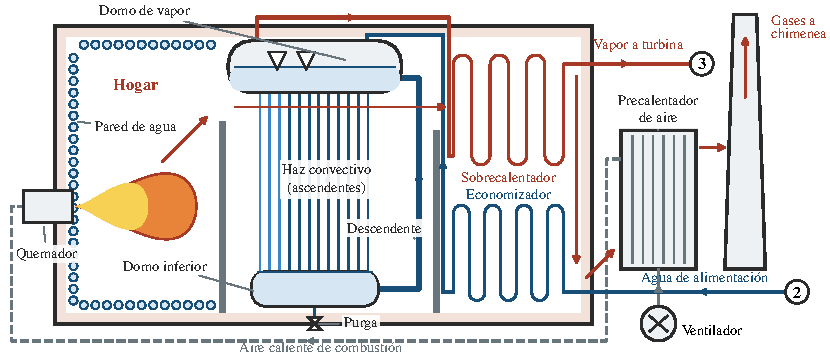
\includegraphics[width=.78\textwidth]{caldero.pdf}
\caption{Dibujo técnico propio, no a escala, de un caldero acuotubular de dos domos: hogar con paredes de agua y quemador, haz convectivo entre domos, descendente, sobrecalentador, economizador, precalentador de aire y chimenea. Azul: agua; rojo: vapor sobrecalentado y gases; gris: aire. La purga se excluye del ciclo cerrado base.}
\label{fig:caldero}
\end{figure*}

\section{Metodología}
\subsection{Diseño del estudio y fronteras}
Se realiza una revisión técnica dirigida de documentación pública de IAPWS, CoolProp, fabricantes y material docente, seguida de modelación determinista. La muestra de Babcock \& Wilcox se utiliza para el contexto accesible, sin atribuir consulta a sus capítulos completos. Las referencias identifican las fuentes utilizadas.

La frontera primaria comprende el circuito agua--vapor de la figura~\ref{fig:ciclo}. Se mantiene la numeración: estado 1, salida del condensador; 2, salida de la bomba; 3, salida del caldero y entrada de la turbina; 4, salida de la turbina. La frontera ampliada incorpora combustible y pérdidas agregadas del caldero. Una tercera extensión convierte trabajo neto de eje en potencia eléctrica mediante un factor supuesto. Las tres fronteras se informan separadamente.

\begin{figure*}[t]
\centering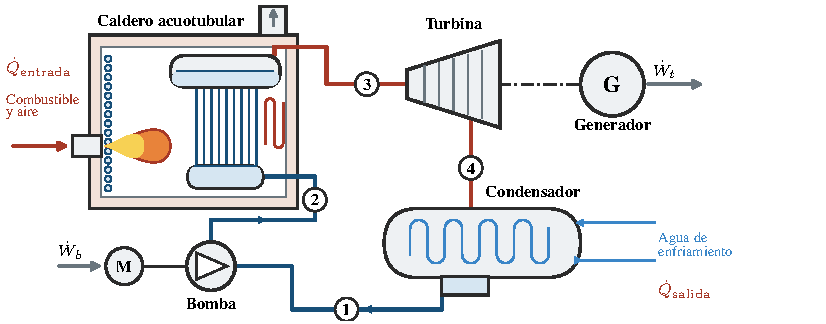
\includegraphics[width=.74\textwidth]{ciclo.pdf}
\caption{Dibujo técnico del ciclo Rankine simple: caldero acuotubular, turbina con generador, condensador de superficie y bomba centrífuga con motor; estados 1--4 y convención de transferencias. El agua conserva un caudal externo de 10 kg/s. El calor de entrada cruza desde la fuente hacia el fluido; el calor rechazado sale al sistema de refrigeración. Elaboración propia.}
\label{fig:ciclo}
\end{figure*}

\subsection{Entradas e hipótesis}
La tabla~\ref{tab:entradas} registra entradas seleccionadas por los autores para el caso analítico. La base de 10 kg/s convierte magnitudes específicas en potencias sin representar una instalación. El estado de 8 MPa y 480~$^\circ$C es subcrítico y sobrecalentado.

\begin{table}[t]
\caption{Entradas del modelo y procedencia}
\label{tab:entradas}
\centering\small
\begin{tabular}{>{\raggedright\arraybackslash}p{.32\columnwidth}>{\raggedright\arraybackslash}p{.20\columnwidth}>{\raggedright\arraybackslash}p{.33\columnwidth}}
\toprule
Magnitud & Valor & Procedencia o condición\\
\midrule
$p_2=p_3$ & 8 MPa & Selección analítica\\
$T_3$ & 480~$^\circ$C & Selección analítica\\
$p_1=p_4$ & 10 kPa & Selección analítica\\
$\dot m$ & 10 kg/s & Base de escala\\
Estado 1 & $x_1=0$ & Líquido saturado supuesto\\
$\eta_t,\eta_b$ ideales & 1; 1 & Reversibilidad interna\\
$\eta_t,\eta_b$ no ideales & 0,85; 0,80 & Escenario supuesto\\
$\eta_{\rm cal}$ & 0,90 & Supuesto sobre PCI\\
PCI del combustible & 50\,000 kJ/kg & Valor nominal supuesto; metano como referencia\\
$\eta_e$ & 0,97 & Conversión neta de eje a electricidad, supuesta\\
\bottomrule
\end{tabular}
\end{table}

Se asume régimen estacionario, agua pura, equilibrio local y variaciones cinéticas y potenciales despreciables. Bomba y turbina son adiabáticas; caldero y condensador carecen de eje. Se omiten pérdidas de presión, fugas, extracciones, purgas, subenfriamiento y auxiliares externos. Todo el circuito comparte $\dot m$; el sistema externo de refrigeración no se dimensiona.

El caso base utiliza bomba y turbina isentrópicas. La variante conserva las condiciones de entrada y añade las eficiencias isentrópicas indicadas, sin representar todas las irreversibilidades de una central. La eficiencia del caldero se aplica después del balance agua--vapor y no modifica estados ya fijados.

\subsection{Propiedades termodinámicas y trazabilidad}
Se utiliza Python con CoolProp \CPversion{} y la cadena de fluido \texttt{IF97::Water}. La documentación distingue este backend de \texttt{Water}, que por defecto emplea otra formulación \cite{coolprop_if97}. Se trabaja internamente con Pa, K, J/kg y J/(kg K), convirtiendo a MPa, grados Celsius y kJ para presentar resultados. La formulación industrial y su implementación se documentan en \cite{iapws,coolprop_paper}.

Para cada estado se fijan dos propiedades independientes. En saturación, $p$ y $T$ están ligados; por ello se añade el título, en vez de pretender que presión y temperatura definan la fracción de vapor. En el líquido comprimido y el vapor sobrecalentado, el título no aplica. La secuencia de resolución es la siguiente.

\subsubsection{Estado 1}
Se fija $p_1=10$ kPa y $x_1=0$. La llamada de saturación devuelve $T_1=\V{IT1}$~$^\circ$C, $h_1=\V{Ih1}\kj$, $s_f$ y $v_f$. El título nulo identifica el extremo líquido saturado.

\subsubsection{Estado 2}
Se fijan $(p_2,s_2)=(8\ \mathrm{MPa},s_1)$ y se resuelve $s(p_2,T_2)=s_1$ por bisección en región líquida. Así se evalúan $h_2$, $v_2$ y $T_2=\V{IT2}$~$^\circ$C sin la pequeña inconsistencia de correlaciones inversas aproximadas. Como control se emplea
\begin{equation}
w_{b,\rm aprox}=v_1(p_2-p_1)=\V{Epump_approx}\kj.
\label{eq:baprox}
\end{equation}
En~\eqref{eq:baprox} se introducen las presiones en kPa. El resultado difiere ligeramente del incremento de entalpía IF97 porque el volumen específico varía con la presión.

\subsubsection{Estado 3}
El par independiente es $(p_3,T_3)=(8\ \mathrm{MPa},480~^\circ\mathrm C)$. Se evalúan directamente $h_3$, $s_3$ y $v_3$ con IF97. La temperatura de saturación a esa presión es \V{ETsatB}~$^\circ$C; por ello el estado es vapor sobrecalentado. Se obtienen $h_3=\V{Ih3}\kj$ y $s_3=\V{Is3}\skj$.

\subsubsection{Estado 4}
Se fijan $(p_4,s_4)=(10\ \mathrm{kPa},s_3)$. Como $s_f<s_3<s_g$ a la presión de condensación, la salida es bifásica. Los extremos de saturación se calculan con el mismo backend y se aplican las relaciones de mezcla:
\begin{align}
x_4&=\frac{s_3-s_f}{s_g-s_f},\label{eq:x}\\
h_4&=h_f+x_4(h_g-h_f),\label{eq:h4}\\
v_4&=v_f+x_4(v_g-v_f).\label{eq:v4}
\end{align}
La sustitución en~\eqref{eq:x} es
\begin{equation}
x_4=\frac{\V{Is3}-\V{EsfC}}{\V{EsgC}-\V{EsfC}}=\V{Ix4}.
\label{eq:xnum}
\end{equation}
Con $h_f=\V{EhfC}\kj$ y $h_g=\V{EhgC}\kj$ resulta $h_4=\V{Ih4}\kj$. El volumen $v_4$ utiliza los mismos extremos $v_f$ y $v_g$; no se evalúa el vapor húmedo como un gas ideal.

Las propiedades proceden de funciones IF97 y reglas de mezcla, sin interpolación manual de tablas. El programa conserva cifras adicionales a las impresas y registra llamadas y conversiones en \texttt{scripts/modelo.py} y en los CSV.

Como control independiente, el caso se resuelve también con las tablas termodinámicas del grupo \cite{tablas_kcha}, con interpolación lineal y $w_b\approx v_1(p_2-p_1)$. Las diferencias de la tabla~\ref{tab:contraste} no superan 0,04~\%.

\begin{table}[t]
\centering
\caption{Contraste de IF97 con las tablas termodinámicas \cite{tablas_kcha}}
\label{tab:contraste}
\begin{tabular}{lrrr}
\toprule
Magnitud & IF97 & Tablas & $\Delta$ [\%]\\
\midrule
$h_1$ [kJ/kg] & 191,81 & 191,83 & +0,009 \\
$h_2$ [kJ/kg] & 199,87 & 199,90 & +0,016 \\
$h_3$ [kJ/kg] & 3349,53 & 3348,60 & -0,028 \\
$h_4$ [kJ/kg] & 2109,33 & 2108,68 & -0,031 \\
$x_4$ [--] & 0,8016 & 0,8014 & -0,027 \\
$\eta$ [\%] & 39,12 & 39,12 & +0,007 \\
\bottomrule
\end{tabular}

\end{table}

\subsection{Balances de masa y energía}
Se toma calor positivo hacia un volumen de control y trabajo de eje positivo cuando sale. La forma estacionaria, sin variaciones cinéticas ni potenciales, es
\begin{align}
\sum\dot m_{\rm ent}&=\sum\dot m_{\rm sal},\label{eq:masa}\\
0&=\dot Q-\dot W+\dot m(h_{\rm ent}-h_{\rm sal}).\label{eq:energia}
\end{align}
Las magnitudes $w_b$ y $q_{\rm sal}$ se informan positivas como consumo de bomba y rechazo térmico, respectivamente. Así, el signo del trabajo de la bomba en~\eqref{eq:energia} es $-\dot W_b$, y el calor del condensador es $-\dot Q_{\rm sal}$. Esta convención evita que una diferencia de signos se interprete como generación de energía.

Para la bomba adiabática, el caldero sin eje, la turbina adiabática y el condensador sin eje se obtiene, respectivamente,
\begin{align}
w_b&=h_2-h_1, &\dot W_b&=\dot m w_b,\label{eq:bomba}\\
q_{\rm ent}&=h_3-h_2, &\dot Q_{\rm ent}&=\dot m q_{\rm ent},\label{eq:caldero}\\
w_t&=h_3-h_4, &\dot W_t&=\dot m w_t,\label{eq:turbina}\\
q_{\rm sal}&=h_4-h_1, &\dot Q_{\rm sal}&=\dot m q_{\rm sal}.\label{eq:condensador}
\end{align}
Por~\eqref{eq:masa}, cada componente conserva 10 kg/s. Los gases y el agua de refrigeración quedan fuera de esa igualdad. Multiplicar kJ/kg por kg/s produce kW.

El trabajo neto y la eficiencia térmica son
\begin{align}
w_{\rm neto}&=w_t-w_b,\label{eq:wn}\\
\eta_{\rm ciclo}&=\frac{w_{\rm neto}}{q_{\rm ent}}
=1-\frac{q_{\rm sal}}{q_{\rm ent}}.\label{eq:eta}
\end{align}
El cierre se comprueba con
\begin{equation}
r_E=q_{\rm ent}-q_{\rm sal}-w_{\rm neto}.
\label{eq:residuo}
\end{equation}
El residuo informa consistencia aritmética y de signos. Como los términos se construyen con las mismas entalpías, su cierre no constituye una validación experimental independiente.

\subsection{Variante con irreversibilidades internas}
El subíndice $s$ identifica una salida isentrópica a la presión de descarga. Para las eficiencias seleccionadas,
\begin{align}
\eta_t&=\frac{h_3-h_{4r}}{h_3-h_{4s}},
&h_{4r}&=h_3-\eta_t(h_3-h_{4s}),\label{eq:etat}\\
\eta_b&=\frac{h_{2s}-h_1}{h_{2r}-h_1},
&h_{2r}&=h_1+\frac{h_{2s}-h_1}{\eta_b}.\label{eq:etab}
\end{align}
Se determinan los estados no ideales con los pares $(p_2,h_{2r})$ y $(p_4,h_{4r})$. En región monofásica se invierte $h(p,T)$ mediante bisección; en mezcla se emplea el título calculado desde la entalpía. Se comprueba además $s_{2r}>s_1$ y $s_{4r}>s_3$, coherente con generación de entropía en equipos adiabáticos. La numeración 1--4 se conserva en ambas variantes; la letra $r$ solo distingue resultados.

\subsection{Eficiencia del caldero y combustible}
El método directo relaciona el calor útil transferido al agua con la potencia química suministrada. Para el circuito sin purga,
\begin{align}
\eta_{\rm cal}&=\frac{\dot m(h_3-h_2)}{\dot m_f\,PCI},\label{eq:etacal}\\
\dot m_f&=\frac{\dot Q_{\rm ent}}{\eta_{\rm cal}PCI},\label{eq:fuel}\\
\eta_{\rm combustible\to eje}&=\eta_{\rm cal}\eta_{\rm ciclo}.\label{eq:global}
\end{align}
El PCI nominal de 50\,000 kJ/kg para metano y $\eta_{\rm cal}=0,90$ son supuestos sobre igual base energética. No representan un combustible analizado. El fabricante diferencia bases caloríficas y efectos del aire \cite{spirax_eficiencia}.

En el método indirecto se cuantifican por separado pérdidas de gases, combustión incompleta, superficies y otras corrientes, con una frontera común:
\begin{equation}
\eta_{\rm cal}=1-
\frac{\sum_j\dot Q_{\text{pérdida},j}}{\dot m_f PCI}.
\label{eq:indirecto}
\end{equation}
Sin composición y temperatura de gases, exceso de aire, humedad, inquemados y temperaturas superficiales no es posible resolver esas pérdidas individualmente. El complemento de 0,90 se informa como pérdida agregada implícita del escenario, no como una medición ni una auditoría por método indirecto.

Para una conversión eléctrica ilustrativa se define $\eta_e=0,97$ aplicada al trabajo neto de eje, después de descontar la bomba. De este modo,
\begin{equation}
\eta_{\text{eléctrica,PCI}}=\eta_e\eta_{\rm cal}\eta_{\rm ciclo}.
\label{eq:electrica}
\end{equation}
La relación no incluye ventiladores, extracción de condensado, tratamiento ni bombeo del sistema de refrigeración. Su resultado es una conversión bajo esa frontera reducida y no una predicción del rendimiento eléctrico neto de una central completa.

\subsection{Sensibilidad y controles numéricos}
Se modifican, una por vez, $T_3=400$, 440, 480, 520 y 560~$^\circ$C; $p_c=5$, 7,5, 10, 15 y 20 kPa; y $p_b=4$, 6, 8, 10 y 12 MPa. Las otras entradas conservan el valor base. Se resuelven ambas variantes en cada punto, manteniendo constantes las eficiencias isentrópicas de la variante no ideal. Esta hipótesis aísla el efecto de las condiciones termodinámicas; no modela el mapa de rendimiento de una turbina comercial.

Se comprueba el dominio IF97, $0<x_4<1$ y $|r_E|<10^{-9}$ kJ/kg. Entalpía, entropía y volumen se contrastan con tres puntos líquidos de la tabla 5 de IAPWS \cite{iapws}, exigiendo error relativo inferior a $10^{-7}$ con el redondeo de referencia. Así se complementa el cierre algebraico.

\section{Resultados}
\subsection{Cuadro completo de estados}
La tabla~\ref{tab:estados} reúne las propiedades del caso ideal. La bomba produce un aumento pequeño de temperatura y una elevación grande de presión. El estado 3 presenta sobrecalentamiento y la expansión termina dentro de la campana. Se evita asignar un título a los estados 2 y 3, donde la mezcla líquido--vapor no define el estado.

\begin{table*}[t]
\caption{Propiedades de los cuatro estados del ciclo ideal calculadas con IF97}
\label{tab:estados}
\centering\small
\begin{tabular}{crrrrrlp{.21\textwidth}}
\toprule
Estado & $p$ [MPa] & $T$ [$^\circ$C] & $h$ [kJ/kg] & $s$ [kJ/(kg K)] & $v$ [m$^3$/kg] & $x$ [--] & Fase\\
\midrule
1 & 0,010 & 45,81 & 191,81 & 0,64922 & 0,001010 & 0,0000 & Líquido saturado \\
2 & 8,000 & 46,07 & 199,87 & 0,64922 & 0,001007 & No aplica & Líquido comprimido \\
3 & 8,000 & 480,00 & 3349,53 & 6,66106 & 0,040365 & No aplica & Vapor sobrecalentado \\
4 & 0,010 & 45,81 & 2109,33 & 6,66106 & 11,760315 & 0,8016 & Mezcla líquido-vapor \\
\bottomrule
\end{tabular}

\end{table*}

El contraste entre $v_4=\V{Iv4}$ y $v_1=\V{Iv1}$ m$^3$/kg explica el pequeño trabajo de compresión del líquido. Las igualdades $s_2=s_1$ y $s_4=s_3$ son hipótesis del modelo ideal.

\subsection{Sustituciones y balance por componente}
La aplicación de~\eqref{eq:bomba}--\eqref{eq:condensador} con las entalpías mostradas conduce a
\begin{align}
w_b&=\V{Ih2}-\V{Ih1}=\V{Iwb}\kj,\label{eq:wbnum}\\
w_t&=\V{Ih3}-\V{Ih4}=\V{Iwt}\kj,\label{eq:wtnum}\\
q_{\rm ent}&=\V{Ih3}-\V{Ih2}=\V{Iqi}\kj,\label{eq:qinum}\\
q_{\rm sal}&=\V{Ih4}-\V{Ih1}=\V{Iqo}\kj.\label{eq:qonum}
\end{align}
Las operaciones se realizan con las cifras internas sin redondear; las sustituciones impresas pueden diferir en la última centésima. El trabajo neto es
\begin{equation}
w_{\rm neto}=\V{Iwt}-\V{Iwb}=\V{Iwn}\kj.
\label{eq:wnnum}
\end{equation}
Con ello,
\begin{equation}
\eta_{\rm ciclo}=\frac{\V{Iwn}}{\V{Iqi}}
\simeq\V{Ietapct}\,\%.
\label{eq:etanum}
\end{equation}

\begin{table}[t]
\caption{Balances del caso ideal y magnitudes de desempeño}
\label{tab:balance}
\centering\small
\begin{tabular}{p{.46\columnwidth}rr}
\toprule
Transferencia & \shortstack{Específica\\{[kJ/kg]}} & \shortstack{Flujo\\{[MW]}}\\
\midrule
Bomba: consumo & \V{Iwb} & \V{IWb}\\
Caldero: calor recibido & \V{Iqi} & \V{IQin}\\
Turbina: trabajo producido & \V{Iwt} & \V{IWt}\\
Condensador: calor rechazado & \V{Iqo} & \V{IQout}\\
Trabajo neto & \V{Iwn} & \V{IWn}\\
\midrule
\multicolumn{2}{l}{Eficiencia térmica del ciclo [\%]} & \V{Ietapct}\\
\multicolumn{2}{l}{Consumo específico de vapor [kg/kWh]} & \V{Isteam_rate}\\
\multicolumn{2}{l}{Trabajo de bomba / turbina [\%]} & \V{Ebwpct}\\
\bottomrule
\end{tabular}
\end{table}

La tabla~\ref{tab:balance} convierte las transferencias a potencia. Por ejemplo,
\begin{equation}
\dot Q_{\rm ent}=
\frac{(10\,\mathrm{kg/s})(\V{Iqi}\,\mathrm{kJ/kg})}{1000}
=\V{IQin}\mww.
\label{eq:potencia}
\end{equation}
El divisor convierte kW a MW. Se conserva $\dot m_1=\dot m_2=\dot m_3=\dot m_4=10$ kg/s, equivalentes a 36\,000 kg/h de vapor.

Con cifras internas, $r_E=\V{Iresidual}$ kJ/kg y $|\dot m r_E|<10^{-11}$ kW. Trabajo neto y calor rechazado recuperan el aporte térmico. Las cifras impresas no conservan la precisión de máquina del cierre.

\subsection{Distribución del calor en el generador}
La separación entre calentamiento sensible, evaporación y sobrecalentamiento se obtiene usando los estados saturados a 8 MPa:
\begin{align}
q_{\rm eco}&=h_f(p_b)-h_2=\V{Eeco}\kj,\label{eq:eco}\\
q_{\rm evap}&=h_g(p_b)-h_f(p_b)=\V{Eevap}\kj,\label{eq:evap}\\
q_{\rm sobre}&=h_3-h_g(p_b)=\V{Esup}\kj.\label{eq:sup}
\end{align}
La suma coincide con $q_{\rm ent}$ y muestra que la evaporación no representa todo el deber térmico. Es una partición termodinámica; asignarla a superficies físicas requiere resolver geometría e intercambio de calor.

Boiler horsepower, BHP, expresa potencia térmica: una BHP equivale aproximadamente a 15,65 kg/h evaporados desde y a 100~$^\circ$C, o 9,81 kW. Para otras condiciones se corrige el caudal con las entalpías de entrada y salida \cite{spirax_capacidad}. Aquí se emplean kg/h y MW.

\subsection{Diagrama temperatura--entropía}
La figura~\ref{fig:ts} contiene campana y trayectorias IF97. Los procesos 1--2 y 3--4 conservan entropía; 2--3 integra calentamiento, evaporación y sobrecalentamiento a 8 MPa; 4--1 condensa a 10 kPa. Se evalúan estados intermedios de cada proceso y dos isóbaras adicionales.

\begin{figure}[t]
\centering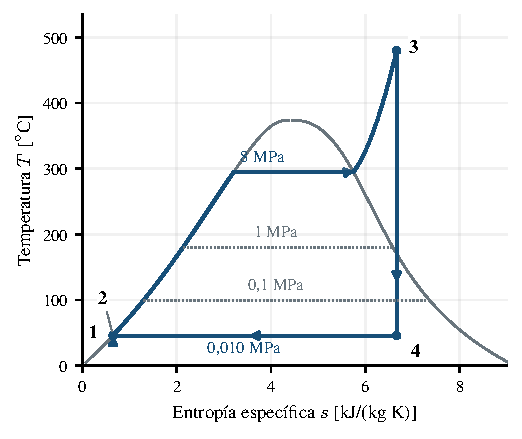
\includegraphics[width=\columnwidth]{ts_ideal.pdf}
\caption{Diagrama $T$--$s$ del ciclo ideal. Estados, campana e isóbaras se calculan con IF97. Las flechas indican el sentido; la separación 1--2 es muy pequeña a esta escala. Las líneas punteadas corresponden a 0,1 y 1 MPa. Elaboración propia.}
\label{fig:ts}
\end{figure}

La expansión termina con $x_4=\V{Ix4}$ y \V{Ehumidity}\,\% de fracción másica líquida. Esa humedad obliga a comprobar la admisibilidad del escape en una turbina específica, aunque el rendimiento resulte favorable.

\subsection{Efecto de las eficiencias isentrópicas}
La tabla~\ref{tab:real} presenta los cuatro estados de la variante no ideal. Las condiciones 1 y 3 permanecen iguales; cambian las salidas de la bomba y la turbina. La bomba requiere \V{Rwb} kJ/kg y la turbina entrega \V{Rwt} kJ/kg. El trabajo neto cae a \V{Rwn} kJ/kg y la eficiencia a \V{Retapct}\,\%, una disminución de \V{Eeta_drop} puntos porcentuales frente al caso ideal.

\begin{table*}[t]
\caption{Estados de la variante no ideal con $\eta_t=0,85$ y $\eta_b=0,80$}
\label{tab:real}
\centering\small
\begin{tabular}{crrrrrlp{.21\textwidth}}
\toprule
Estado & $p$ [MPa] & $T$ [$^\circ$C] & $h$ [kJ/kg] & $s$ [kJ/(kg K)] & $v$ [m$^3$/kg] & $x$ [--] & Fase\\
\midrule
1 & 0,010 & 45,81 & 191,81 & 0,64922 & 0,001010 & 0,0000 & Líquido saturado \\
2 & 8,000 & 46,56 & 201,89 & 0,65552 & 0,001007 & No aplica & Líquido comprimido \\
3 & 8,000 & 480,00 & 3349,53 & 6,66106 & 0,040365 & No aplica & Vapor sobrecalentado \\
4 & 0,010 & 45,81 & 2295,36 & 7,24430 & 12,901152 & 0,8794 & Mezcla líquido-vapor \\
\bottomrule
\end{tabular}

\end{table*}

La potencia neta es \V{RWn} MW y el calor rechazado, \V{RQout} MW. El aumento de $h_{4r}$ reduce trabajo y eleva el título a \V{Rx4}. El residuo es $\V{Rresidual}$ kJ/kg.

\subsection{Consumo y frontera del combustible}
El caso ideal requiere \V{Ifuel} kg/s de combustible nominal: \V{IfuelMW} MW químicos y \V{EboilerlossMW} MW de pérdida agregada del caldero. El rendimiento combustible--eje es \V{Ietafuelpct}\,\%. La conversión eléctrica supuesta produce \V{IelectricMW} MW y \V{Ietaelecpct}\,\% sobre PCI.

La variante consume \V{Rfuel} kg/s y alcanza \V{Retafuelpct}\,\% combustible--eje; con conversión eléctrica, \V{Retaelecpct}\,\% y \V{RelectricMW} MW. El consumo ligeramente menor a caudal fijo proviene del mayor aporte de la bomba al agua; no indica una mejora, pues cae la potencia útil.

\subsection{Sensibilidad a las condiciones de operación}
La figura~\ref{fig:sens} y las tablas~\ref{tab:temp}--\ref{tab:pb} muestran el barrido determinista. Cada fila corresponde a un nuevo cierre completo del ciclo. No se suman los efectos de barridos independientes para representar una condición combinada.

\begin{figure*}[t]
\centering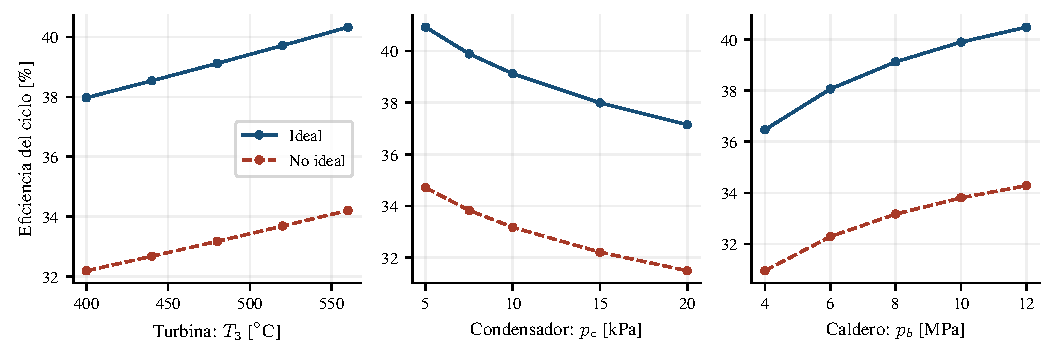
\includegraphics[width=\textwidth]{sensibilidad.pdf}
\caption{Eficiencia térmica frente a una variable por vez. Se mantienen las demás entradas en su condición base. Ambas variantes conservan sus eficiencias isentrópicas en todos los puntos. Elaboración propia a partir de IF97.}
\label{fig:sens}
\end{figure*}

\begin{table}[t]
\caption{Sensibilidad ideal a $T_3$, con $p_b=8$ MPa y $p_c=10$ kPa}
\label{tab:temp}
\centering\small
\begin{tabular}{rrrr}
\toprule
$T_3$ [$^\circ$C] & $\eta$ [\%] & $w_{\rm neto}$ [kJ/kg] & $x_4$\\
\midrule
400 & 37,97 & 1116,14 & 0,7622 \\
440 & 38,54 & 1174,38 & 0,7830 \\
480 & 39,12 & 1232,14 & 0,8016 \\
520 & 39,72 & 1290,35 & 0,8187 \\
560 & 40,33 & 1349,51 & 0,8347 \\
\bottomrule
\end{tabular}

\end{table}

Al elevar $T_3$ de 400 a 560~$^\circ$C, la eficiencia ideal pasa de \V{STloeta} a \V{SThieta}\,\%, el trabajo de \V{STlown} a \V{SThiwn} kJ/kg y el título de \V{STlox} a \V{SThix}. La variante no ideal alcanza $x_4=\V{SThixR}$. El sobrecalentamiento beneficia conversión y calidad final.

\begin{table}[t]
\caption{Sensibilidad ideal a $p_c$, con $p_b=8$ MPa y $T_3=480~^\circ$C}
\label{tab:pc}
\centering\small
\begin{tabular}{rrrr}
\toprule
$p_c$ [kPa] & $\eta$ [\%] & $w_{\rm neto}$ [kJ/kg] & $x_4$\\
\midrule
5 & 40,92 & 1311,04 & 0,7811 \\
7,5 & 39,89 & 1265,52 & 0,7929 \\
10 & 39,12 & 1232,14 & 0,8016 \\
15 & 37,99 & 1183,46 & 0,8144 \\
20 & 37,14 & 1147,71 & 0,8239 \\
\bottomrule
\end{tabular}

\end{table}

Reducir $p_c$ de 20 a 5 kPa eleva la eficiencia de \V{SChieta} a \V{SCloeta}\,\% y el trabajo de \V{SChiwn} a \V{SClown} kJ/kg. El título cae de \V{SChix} a \V{SClox}: aumentan humedad y exigencia de vacío. La viabilidad de 5 kPa depende del ambiente y del condensador.

\begin{table}[t]
\caption{Sensibilidad ideal a $p_b$, con $p_c=10$ kPa y $T_3=480~^\circ$C}
\label{tab:pb}
\centering\small
\begin{tabular}{rrrr}
\toprule
$p_b$ [MPa] & $\eta$ [\%] & $w_{\rm neto}$ [kJ/kg] & $x_4$\\
\midrule
4 & 36,46 & 1168,39 & 0,8511 \\
6 & 38,06 & 1209,20 & 0,8228 \\
8 & 39,12 & 1232,14 & 0,8016 \\
10 & 39,89 & 1244,99 & 0,7843 \\
12 & 40,47 & 1251,21 & 0,7693 \\
\bottomrule
\end{tabular}

\end{table}

Elevar $p_b$ de 4 a 12 MPa aumenta la eficiencia de \V{SBloeta} a \V{SBhieta}\,\% y el trabajo de \V{SBlown} a \V{SBhiwn} kJ/kg. El título baja de \V{SBlox} a \V{SBhix}. La humedad puede justificar recalentamiento o menor presión, pese a la ganancia de rendimiento.

\section{Discusión}
\subsection{Interpretación del rendimiento}
El ciclo convierte \V{Ietapct}\,\% del calor recibido en trabajo y rechaza \V{Erejected_pct}\,\%. El rechazo ocurre en el condensador y se distingue de las pérdidas del caldero. Aprovecharlo como calor de proceso exige redefinir la frontera mediante cogeneración.

La relación de trabajo de bomba a turbina, \V{Ebwpct}\,\%, define la diferencia entre potencia bruta y neta. La menor caída útil de entalpía en la turbina domina la reducción no ideal. Su eficiencia isentrópica caracteriza al componente y no equivale a $\eta_{\rm ciclo}$.

Como control de segunda ley, el límite de Carnot entre la temperatura máxima del fluido y la temperatura de condensación es
\begin{equation}
\eta_{\rm Carnot}=1-\frac{T_1}{T_3}=\V{Ecarnot}\,\%.
\label{eq:carnot}
\end{equation}
Se introducen temperaturas en kelvin. El rendimiento Rankine es menor porque una parte importante del calor se añade por debajo de $T_3$. Para la trayectoria reversible de calentamiento del agua, su temperatura media termodinámica de adición es
\begin{equation}
\overline T_{\rm ent}=\frac{q_{\rm ent}}{s_3-s_2}
=\V{ETmean}\,\mathrm K.
\label{eq:tmedia}
\end{equation}
Esta temperatura caracteriza el calentamiento reversible del fluido. Evaluar exergía del combustible exigiría además definir el ambiente y la fuente térmica.

\subsection{Comparación con documentación técnica}
Se repite el modelo a las condiciones de Carmichael: 3 MPa, 460~$^\circ$C y 7,384 kPa. IF97 entrega \V{Metapct}\,\% y $x_4=\V{Mx}$, frente a 35,9\,\% y 0,851 de sus tablas \cite{mit_rankine}. El rendimiento coincide al redondeo; el título difiere ligeramente por las propiedades de origen. Sus barridos respaldan las tendencias de presión y sobrecalentamiento \cite{mit_parametros}.

La EPA informa rendimientos eléctricos de hasta 45\,\% sobre PCS y un promedio cercano a 33\,\% para el conjunto de grandes sistemas descrito \cite{epa}. Constituyen una referencia de escala: nuestro \V{Ietapct}\,\% usa calor del agua como denominador y el \V{Retaelecpct}\,\% eléctrico utiliza PCI y omite auxiliares. Las fronteras impiden una comparación porcentual directa con esas centrales.

La selección industrial también considera humedad, corrosión y materiales. El recalentamiento modifica la expansión y la regeneración eleva la temperatura de alimentación. Ambas opciones pueden mejorar el ciclo, pero añaden estados y requieren nuevos balances.

\subsection{Refrigeración, combustible y escalamiento}
El condensador ideal debe transferir \V{IQout} MW al medio externo. Para mostrar su escala, si se supone agua de refrigeración con $c_p=4,18$ kJ/(kg K) y un incremento de 10 K, el caudal necesario por balance sensible es
\begin{equation}
\dot m_{\rm ref}=\frac{\dot Q_{\rm sal}}{c_p\Delta T}
=\V{Ecoolwater}\,\mathrm{kg/s}.
\label{eq:ref}
\end{equation}
La estimación no determina la reposición de una torre. Disponibilidad de agua y aproximación térmica restringen la disminución de $p_c$.

Potencias y calores escalan con $\dot m$ si estados y eficiencias permanecen constantes. En equipos reales cambian pérdidas, transferencia y auxiliares con la carga. Por ello 10 kg/s proporciona una escala de potencia, sin dimensionar la instalación.

Reducir pérdidas del caldero mejora el rendimiento respecto del combustible sin cambiar $\eta_{\rm ciclo}$ a estados fijos. Variar el PCI modifica el consumo másico; mezclarlo con PCS introduciría diferencias de denominador, no mejoras físicas.

\section{Operación, aplicaciones y límites del equipo}
\subsection{Combustión, medición y control}
Para metano, $\mathrm{CH_4+2O_2\to CO_2+2H_2O}$ define el oxígeno teórico. El factor $\lambda=\dot m_{\rm aire}/\dot m_{\rm aire,esteq}$ expresa el aire relativo al estequiométrico. Poco aire favorece combustión incompleta y demasiado incrementa el calor evacuado con gases. Sin datos de gases no se optimiza $\lambda$.

Medir presión, temperatura y caudales de agua, vapor y combustible permite contrastar el balance. Indicadores de nivel, manómetros y termómetros sostienen la operación; detectores de llama y válvulas de seguridad aportan protección. Estas últimas no sustituyen la regulación de presión.

El control de un elemento mide nivel; el de dos añade caudal de vapor; el de tres incorpora alimentación para compensar variaciones de demanda y suministro \cite{spirax_control}. La expansión o contracción de burbujas altera el nivel aparente. Alarmas de bajo nivel y vigilancia de llama añaden barreras de protección \cite{spirax_nivel}.

Arranque y parada requieren controlar gradientes térmicos, expansión, drenajes e inventario según el equipo. Son transitorios excluidos del cálculo; el cierre estacionario no demuestra su seguridad.

\subsection{Agua, depósitos y purgas}
Depósitos de dureza añaden resistencia térmica; oxígeno y química inadecuada favorecen corrosión. El arrastre transporta agua y contaminantes al vapor. Ablandamiento, desmineralización y desaireación forman parte del tratamiento externo; el interno depende de presión y materiales \cite{spirax_agua}. No existen dosis universales para este modelo.

La purga continua controla sólidos disueltos y la de fondo retira sedimentos; la conductividad ayuda al control \cite{spirax_purga}. Al incluir purga, cambian los balances:
\begin{align}
\dot m_{\rm alim}&=\dot m_v+\dot m_{\rm purga},\label{eq:purga_m}\\
\dot Q_{\rm agua}&=\dot m_v(h_3-h_2)
 +\dot m_{\rm purga}(h_{\rm purga}-h_2).\label{eq:purga_e}
\end{align}
Para líquido saturado a 8 MPa y purga del 2\,\% del vapor, el término adicional de~\eqref{eq:purga_e} es \V{Epurge_extra} MW. Es una extensión local con igual $h_2$, excluida del caso base; una planta completa requiere reposición y posible recuperación de calor.

\subsection{Aplicaciones, mantenimiento y seguridad}
Las aplicaciones comprenden generación eléctrica, cogeneración azucarera y papelera, procesos petroquímicos y usos mineros según la demanda térmica. La propulsión naval puede utilizar turbinas de vapor. Los HRSG aprovechan calor residual en ciclos combinados. Cada aplicación exige ajustar presiones, combustible y objetivo de producción.

La adaptación a presión elevada y la flexibilidad de superficies se acompañan de inversión, exigencia de agua y mantenimiento. Un inventario menor no elimina el riesgo de presión. La selección frente a un pirotubular depende de demanda, continuidad y costo de vida útil.

El mantenimiento incluye limpieza, inspección de tubos, revisión de protecciones y química. Espesores y temperaturas apoyan el seguimiento predictivo. Roturas, sobrecalentamiento y corrosión requieren investigar la causa; perder eficiencia no identifica por sí solo el mecanismo de falla.

ASME BPVC.I-2025 trata la construcción de calderos de potencia \cite{asme}; se consulta su ficha, sin certificar un diseño con el código completo. La Ley 29783 aporta el marco peruano de seguridad y salud laboral \cite{ley}. Inspecciones y pruebas hidrostáticas requieren criterios aplicables al equipo; este balance no prescribe presiones de ensayo.

\subsection{Alcances de la evidencia}
La sensibilidad es determinista, sin significancia estadística. No se modelan variaciones de eficiencia con carga, emisiones, costos, dimensiones ni tensiones. Resolver propiedades no demuestra viabilidad de planta.

La siguiente extensión requiere mediciones con incertidumbre instrumental y una frontera acordada, antes de añadir auxiliares, purgas, pérdidas de presión, recalentamiento y regeneración.

\section{Conclusiones}
Para 8 MPa, 480~$^\circ$C, 10 kPa y 10 kg/s, el balance de los cuatro componentes entrega \V{IWn} MW y \V{Ietapct}\,\% de eficiencia ideal. El residuo es menor que $10^{-9}$ kJ/kg.

Con eficiencias isentrópicas de 0,85 y 0,80, los resultados bajan a \V{RWn} MW y \V{Retapct}\,\%. El título ideal de \V{Ix4} exige revisar la humedad admisible; el cierre numérico no basta para seleccionar una turbina.

El sobrecalentamiento mejora eficiencia, trabajo y título. Reducir presión de condensación o elevar presión de caldero mejora rendimiento, pero aumenta humedad. La selección debe integrar refrigeración y límites del equipo.

Con 90\,\% de eficiencia del caldero sobre PCI, el rendimiento combustible--eje ideal es \V{Ietafuelpct}\,\%. Son escenarios analíticos sin mediciones; agua, control y mantenimiento requieren evaluación adicional para sostener esas condiciones.

\bibliographystyle{IEEEtran}
\bibliography{referencias}
\end{document}
